\documentclass[a4paper, 12pt]{article}

\usepackage{hyperref}
\usepackage[warn]{mathtext}
\usepackage[utf8]{inputenc}
\usepackage[T2A]{fontenc}
\usepackage[english,russian]{babel}
\usepackage{multirow}
\usepackage{float}
\restylefloat{table}
\usepackage{amsmath,amsfonts,amssymb,amsthm,mathtools}
\usepackage{indentfirst}
\DeclareSymbolFont{T2Aletters}{T2A}{cmr}{m}{it}
\usepackage{ gensymb }
\mathtoolsset{showonlyrefs=true}
\usepackage{euscript}
\usepackage{mathrsfs}
\usepackage[left=2cm,right=2cm,top=2cm,bottom=2cm]{geometry}
\usepackage{graphicx}
\usepackage{wrapfig}
\usepackage[rgb]{xcolor}
\hypersetup{
colorlinks=true,
urlcolor=blue
}
\usepackage{tikz}

\title{Лабораторная работа}
\author{Гисич Арсений Б03-102}
\date{2022}

\begin{document}

	\begin{center}
		{\large МОСКОВСКИЙ ФИЗИКО-ТЕХНИЧЕСКИЙ ИНСТИТУТ (НАЦИОНАЛЬНЫЙ ИССЛЕДОВАТЕЛЬСКИЙ УНИВЕРСИТЕТ)}
	\end{center}
	\vspace{5 cm}
	{\Large
		\begin{center}
			{\bf Лабораторная работа 3.4.5}\\[0.2 cm]
			Петля гистерезиса (динамический метод)
		\end{center}
	}
	\vspace{4 cm}
	\begin{flushright}
		{\Large Выполнил: \\
			\vspace{0.2 cm}
			Гисич Арсений \\
			\vspace{0.2 cm}
			Б03-102 \\}
	\end{flushright}
	\vspace{9 cm}
	\begin{center}
		Долгопрудный\\[0.1 cm]
		2022
	\end{center}
\thispagestyle{empty}

\section{Аннотация}

В данной работе изучались петли гистерезиса различных ферромагнитных материалов в переменных полях.

\section{Теоретические сведения}

Основные характеристики
ферромагнетиков — их коэрцитивное поле $H_c$, магнитная проницаемость
$\mu$, рассеиваемая в виде тепла при перемагничивании мощность — зависят
от частоты перемагничивающего поля. В данной работе кривые гистерезиса ферромагнитных материалов изучаются в поле частоты $\nu_0 = 50~Гц$
с помощью электронного осциллографа.

\begin{figure}[H]
\begin{center}
    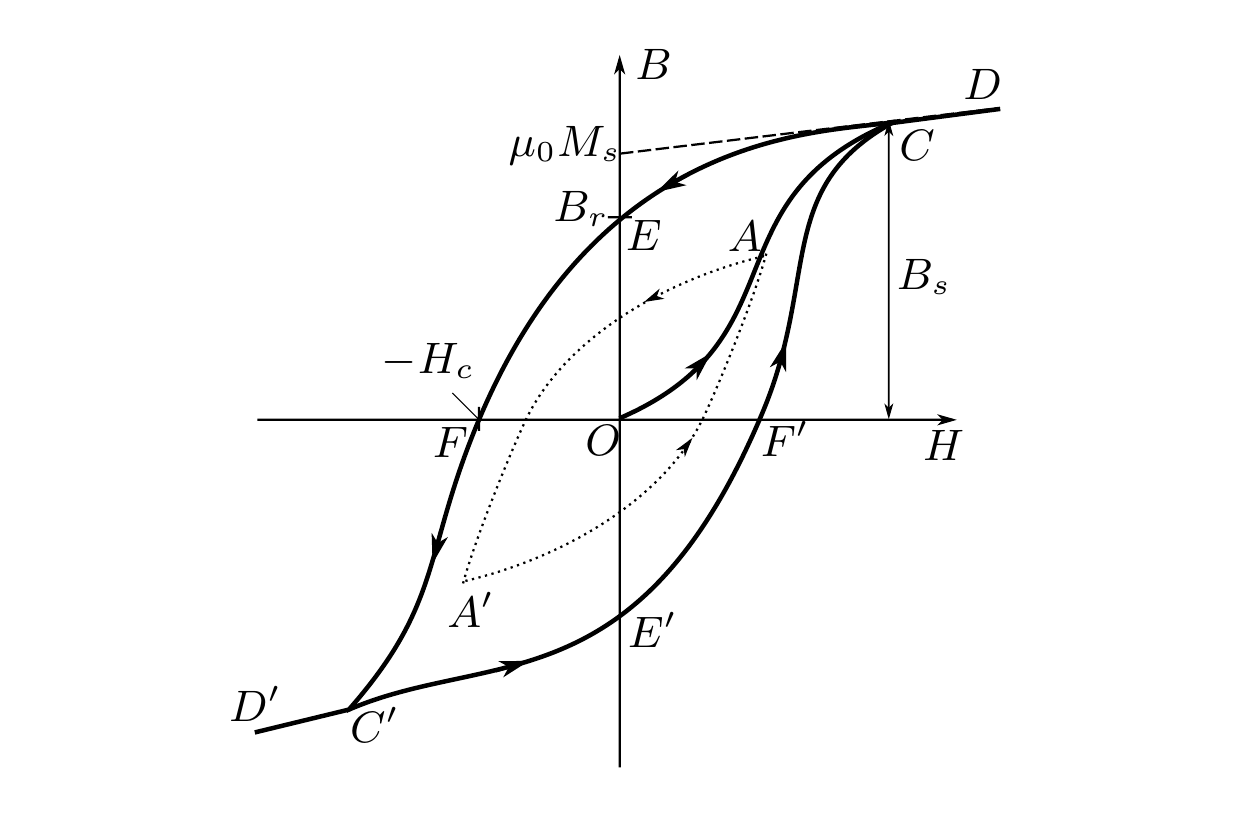
\includegraphics[scale=2]{1.png}
\end{center}
\caption{Петля гистерезиса ферромагнетика}
\label{fig:petlya}
\end{figure}

Магнитная индукция $ B $ и напряжённость поля $ H $ в ферромагнитном материале неоднозначно связаны между собой: индукция зависит
не только от напряжённости, но и от предыстории образца. Связь между $ B $ и $ H $ типичного ферромагнетика иллюстрирует рис.~\ref{fig:petlya}.

Если к ферромагнитному образцу прикладывать переменное внешнее
магнитное поле, то его состояние на плоскости $ B-H $ будет изменяться
по замкнутой кривой — петле гистерезиса. Размер петли определяется
максимальным значением напряжённости $ H $ в цикле (например, петля $ AA' $,
обозначенная пунктиром на рис.~\ref{fig:petlya}). Если амплитуда напряжённости достаточно велика, то образец будет периодически достигать насыщения,
что на рисунке соответствует кривой $ CEFC'E'F'C $ (предельная петля
гистерезиса). Пересечение предельной петли с вертикальной осью соответствует остаточной индукции $B_r$, пересечение с горизонтальной осью
— коэрцитивному полю $H_c$. Крайние точки петель, соответствующие амплитудным значениям $ H $ (например, точка $ A $ на рис.~\ref{fig:petlya}), лежат на начальной кривой намагничивания ($ OAC $).

\textbf{Измерение магнитной индукции.} Магнитную индукцию $ B $ удобно
определять с помощью ЭДС, возникающей при изменении магнитного
потока $ \Phi $ в катушке, намотанной на образец. Пусть катушка c $ N $ витками плотно охватывает образец сечением $ S $, и индукция $ B $ в образце
однородна. Тогда

\begin{equation}
|B|=\frac{1}{SN}\int\mathcal{E} dt.
\label{eq:|B|}
\end{equation}
\begin{wrapfigure}{r}{0.35\linewidth}
	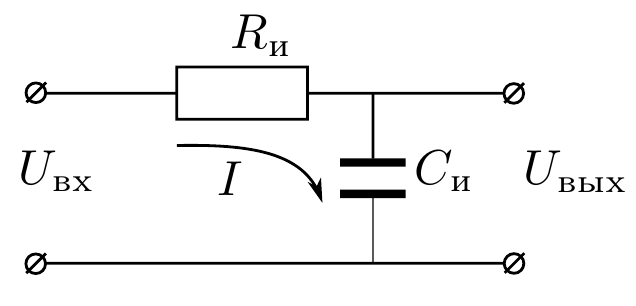
\includegraphics[width=\linewidth]{2.png}
	\caption{Интегрирующая ячейка}
	\label{fig:int}
\end{wrapfigure}

Для интегрирования в работе используется интегрирующая $ RC $-цепочка (рис.~\ref{fig:int}).
«Входное» напряжение от источника $U_{\text{вх}}(t)$ подаётся на последовательно соединённые резистор $R_\text{и}$ и конденсатор $C_\text{и}$. <<Выходное>>
напряжение $U_{\text{вых}}(t)$ снимается с конденсатора. Предположим, что 1) сопротивление источника мало по сравнению с $R_\text{и}$, 2) выходное сопротивление (сопротивление на входе осциллографа), напротив, велико: $R_{\text{вых}}$ $ \gg $ $R_\text{и}$ и, наконец, 3) сопротивление $R_\text{и}$ достаточно велико, так что почти всё падение напряжения приходится на него, а $U_{\text{вых}}$ $\ll$ $U_{\text{вх}}$. В таком случае ток цепи равен I = ($U_{\text{вх}}$ - $U_{\text{вых}}$)/$R_\text{и}$ $\approx$ $U_{\text{вх}}$/$R_\text{и}$, и входное и выходное сопротивление связаны соотношением
\begin{equation}
U_{\text{вых}} = \frac{q}{C_\text{и}} = \frac{1}{C_\text{и}}\int\limits_0^t Idt \approx \frac{1}{\tau_\text{и}} \int\limits_0^t U_{\text{вх}}dt,
\label{eq:U_ext}
\end{equation}
где $\tau_\text{и}=R_\text{и}C_\text{и}$ - постоянная времени $ RC $ - цепочки. Для индукции поля из ($\ref{eq:|B|}$) получаем 
\begin{equation}
|B|=\frac{1}{SN}\int U_{\text{вх}} dt=\frac{\tau_\text{и}}{SN}U_{\text{вых}}.
\label{eq:|B|new}
\end{equation}

\textbf{Замечание.} Уточним критерий применимости соотношения \eqref{eq:U_ext}. Пусть на вход интегрирующей ячейки подан синусоидальный сигнал с частотой $\omega_0$. Тогда, пользуясь методом комплексных амплитуд, нетрудно найти отношение амплитуд входного и выходного напряжений:
\begin{equation}
\frac{U_{\text{вых}}}{U_{\text{вх}}}=\frac{1/\omega_0C}{\sqrt{R^2+1/(\omega_0C)^2}}.
\end{equation}
Тогда неравенство $U_{\text{вых}} \ll U_{\text{вх}}$ реализуется, если 
\begin{equation}
\tau \equiv RC\gg \frac{1}{\omega_0}
\end{equation}
(импеданс конденсатора мал по сравнению сопротивлением резистора).
В таком случае для синусоидального сигнала имеем
\begin{equation}
\frac{U_{\text{вых}}}{U_{\text{вх}}}\approx\frac{1}{\omega_0\tau}.
\end{equation}
В общем случае, если $\omega_0$ — частота самой низкой гармоники в спектре
произвольного входного сигнала, то при $\omega_0\tau \gg 1$ неравенство $U_{\text{вых}} \ll U_{\text{вх}}$ выполняется на любой частоте $\omega > \omega_0$.

\section{Методика измерений}

Схема установки изображена на рис.~\ref{fig:scheme}. Напряжение сети (220 В,
50 Гц) с помощью трансформаторного блока Т, состоящего из регулировочного автотрансформатора и разделительного понижающего трансформатора, подаётся на намагничивающую обмотку $N_0$ исследуемого образца.
\begin{figure}[h!]
	\centering
	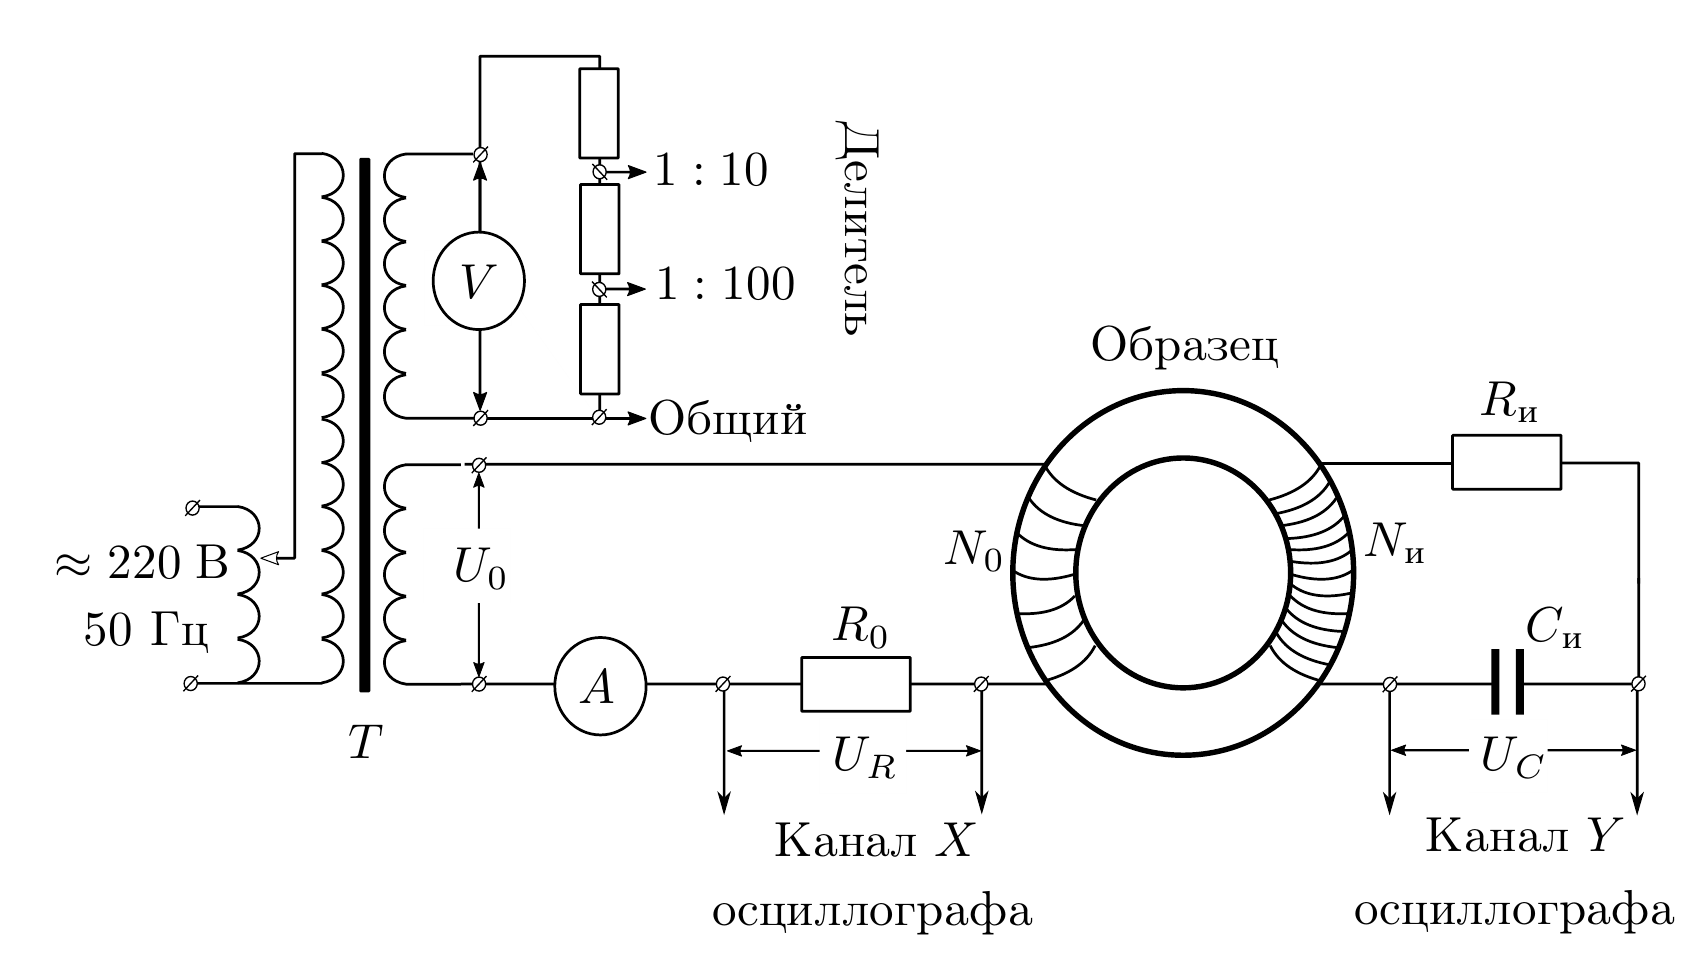
\includegraphics[scale=2]{3.png}
	\caption{ Схема установки для исследования намагничивания образцов}
	\label{fig:scheme}
\end{figure}

В цепь намагничивающей катушки, на которую подаётся некоторое
напряжение $U_0$, последовательно включено сопротивление $R_0$. Напряжение на $R_0$, равное $U_R = R_0I_0$, где $I_0$ — ток в намагничивающей обмотке $N_0$, подаётся на канал $ X $ осциллографа. Связь напряжённости $ H $ в
образце и тока $I_0$ рассчитывается по теореме о циркуляции. 
Действующее значение переменного тока в обмотке $N_0$ измеряется амперметром A.
Для измерения магнитной индукции $ B $ с измерительной обмотки $N_\text{и}$
на вход $ RC $-цепочки подаётся напряжение $U_\text{и}$ ($U_{\text{вх}}$), пропорциональное
производной $ dB/dt $. С интегрирующей ёмкости $C_\text{и}$ снимается напряжение $U_C$ ($U_{\text{вых}}$), пропорциональное величине $ B $, и подаётся на вход $ Y $
осциллографа. Значение индукции поля $ B $ рассчитывается по формуле \eqref{eq:|B|new}.
Замкнутая кривая, возникающая на экране, воспроизводит в некотором масштабе (различном для осей $ X $ и $ Y $) петлю гистерезиса. Чтобы придать этой кривой количественный смысл, необходимо установить
масштабы изображения, т. е. провести калибровку каналов $ X $ и $ Y $ осциллографа.
  	
\section{Используемое оборудование}

\begin{enumerate}
    \item автотрансформатор;
    \item понижающий трансформатор;
    \item интегрирующая цепочка;
    \item амперметр;
    \item вольтметр;
    \item электронный осциллограф;
    \item делитель напряжения;
    \item тороидальные образцы с двумя обмотками.
\end{enumerate}

\section{Результаты измерений и обработка данных}

Параметры установки:
\begin{description}
\item{} $R = 3,5~Ом$
\item{} $R_1 = 1008~Ом$
\end{description}

\begin{table}[h!]
\begin{center}
\begin{tabular}{|c|c|c|c|}
\hline
$\nu, кГц$ & $\delta_{\nu}, кГц$ & $U, B$  & $\delta_U, B$ \\ \hline
31,38  & 0,01    & 0,682 & 0,001 \\ \hline
31,44  & 0,01    & 0,715 & 0,001 \\ \hline
31,51  & 0,01    & 0,765 & 0,001 \\ \hline
31,58  & 0,01    & 0,822 & 0,001 \\ \hline
31,69  & 0,01    & 0,910 & 0,001 \\ \hline
31,73  & 0,01    & 0,951 & 0,001 \\ \hline
31,78  & 0,01    & 0,992 & 0,001 \\ \hline
32,08  & 0,01    & 1,187 & 0,001 \\ \hline
32,86  & 0,01    & 0,705 & 0,001 \\ \hline
32,81  & 0,01    & 0,735 & 0,001 \\ \hline
32,68  & 0,01    & 0,825 & 0,001 \\ \hline
32,48  & 0,01    & 0,986 & 0,001 \\ \hline
32,30  & 0,01    & 1,127 & 0,001 \\ \hline
32,12  & 0,01    & 1,189 & 0,001 \\ \hline
\end{tabular}
\end{center}
\caption{Амплитудно-частотная характеристика колебательного контура для 1-ой ёмкости}
\label{tab2}
\end{table}

\section{Обсуждение результатов и выводы}

В данной работе был исследован резонанс токов в параллельном колебательном контуре с изменяемой ёмкостью, были определены параметры контура, получены амплитудно-частотные и фазово-частотные характеристики контура при 2 различных значениях ёмкости конденсатора.  По графику АЧХ были определены добротности соответствующих контуров. Полученные значения:
$$ Q_1 = 29\pm1, \quad Q_7 = 16\pm1. $$
Также добротности были определены с помощью графика ФЧХ 2-мя способами. Значения, полученные 1-ым способом (по углу наклона прямой вблизи резонанса):
$$ Q_1 = 18\pm5, \quad Q_7 = 13\pm4. $$
Результат, полученный 2-ым способом (по расстоянию между y(-1/4) и y(1/4) по оси x):
$$ Q_1 = 17\pm1, \quad Q_7 = 13\pm1. $$
Значения добротности, рассчитанные теоретически:
$$ Q_1 = 30, \quad Q_7 = 17. $$
Результат, рассчитанный по АЧХ совпадает с теоретическим в пределах погрешности. Однако результаты, полученные при исследовании ФЧХ, совпадают по порядку, но существенно отличаются от рассчитанных теоретически. Это может быть связано с высокой погрешностью предложенного метода измерения сдвига фаз между $E$ и $U$ ввиду его сложности. Например, графики ФЧХ для обоих контуров не пересекают прямую $y = -1/4$, что говорит о наличии систематической погрешности измерений.

Также была определена зависимость активного сопротивления катушки $R_L$ от резонансной частоты $\nu_0$. Как видно из графика, $R_L$ возрастает с возрастанием частоты. Это может быть вызвано скин-эффектом. Резкое скачкообразное изменение значений $R_L$ может быть связано с изменением амплитуды ЭДС в процессе эксперимента.

\end{document}
